\documentclass[a4paper]{article}

\usepackage[english]{babel}
\usepackage[utf8]{inputenc}
\usepackage{amsmath}
\usepackage{graphicx}
\usepackage[colorinlistoftodos]{todonotes}

\title{TIPNet \\ (Temporal Information Partitioning Network)}

\author{Allison Goodwell}

\date{\today}

\begin{document}
\maketitle

\section{Introduction}

This Matlab interface takes inputs of time-series datasets as ``nodes'' in a network, and computes information measures to identify and characterize time dependencies between nodes.

\subsection{Quick Start}
Run the file called EntropyGUI\_mainwindow.m.  Click Load New Data option, and load either a .mat or .xls file containing columns of time series data.  For a .xls file, variable names should be the top row of the file.  A .mat file should include a (\# variables x \# timesteps) matrix called ``data'' and a (1 x \# variables)  cell called \textit{varnames} with variable names.  For any processing or \textit{pdf} options, see the appropriate section.  To compute the network, click on Compute Links.  All results are stored in the entropy structure that is saved in the project file.  Results can be viewed by clicking Plot Results.

\begin{figure}[h!]\label{fig:start}
\begin{center}
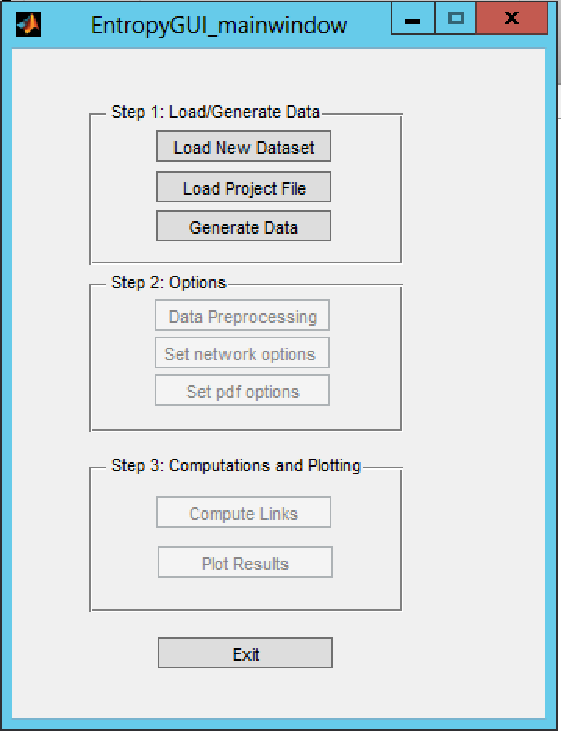
\includegraphics[scale=.5]{Image_PreLoad.pdf}
\caption{Main screen, one of first 3 buttons must be chosen to load data or project file, or generate test data.}
\end{center}
\end{figure}

\begin{figure}[h!]\label{fig:start}
\begin{center}
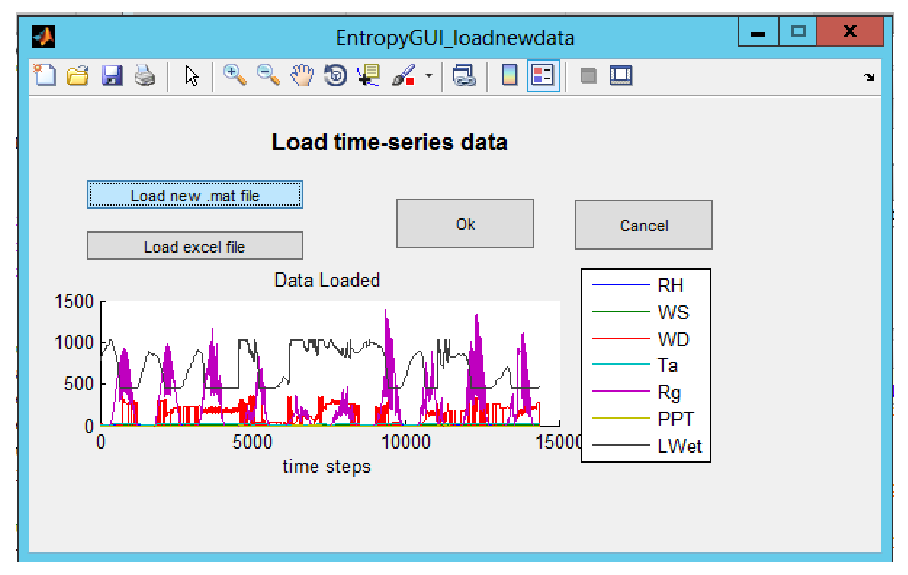
\includegraphics[scale=.5]{Image_LoadData.pdf}
\caption{Example weather station data set loaded as a .mat file}
\end{center}
\end{figure}

\section{Information Measures}
\label{sec:measures}

\subsection{Entropy and Mutual Information}

\begin{equation}
H(X)= -\sum p(x) \log_2(p(x))
\end{equation}
 
\begin{equation}
I(X;Y) = H(Y) - H(Y|X) = \sum p(x,y) \log_2\left(\frac{p(x,y)}{p(x)p(y)}\right)
\end{equation}

\noindent
where $X$ and $Y$ are time-series variables that may be simultaneous or involve some time lag between them.  When we consider $X$ to be a ``source'' node and $Y$ to be a ``target'' node, the quantity $I(X;Y)$ indicates the strength of a link from $X$ to $Y$ in that $X$ reduces the uncertainty of the $Y$.  For a range of lag times $\tau$, $I(X(t-\tau);Y)$ is computed.  Transfer Entropy $T_E(X(t-\tau) \rightarrow Y)$, which is equivalent to the conditional information $I(X(t-\tau);Y|Y(t-1))$ is also computed as follows:

\begin{equation}\label{eq:T}
I(X;Y|Y_1) = \sum_{x,y,y_\tau} p(x,y,y_1)\log\left[\frac{p(x,y,y_1)}{p(y,y_1)}\right]
\end{equation} 

where abbreviated symbols are $x=x(t-\tau)$, $y = y(t)$, and $y_1 = y(t-1)$.  As discussed in \cite{Goodwell2015}, $T_E$ omits a redundant component (overlapping information shared to target $Y(t)$ by both $X(t-\tau)$ and $Y(t-1)$) but adds in a synergistic component (information shared to the target $Y(t)$ due to knowledge of both sources together).

The dominant time scale of the link from $X$ to $Y$ is the $\tau>0$ corresponding either to the maximum $I(X(t-\tau);Y)$ (bits) or the normalized value $\frac{I(X(t-\tau);Y)}{min(H(X),H(Y))}$ (bits/bit), depending on the \textbf{mi.NormOpt} parameter (see next section).  

\subsection{PDF estimation and statistical significance}
Computation of these measures involves estimating joint probability density functions (\textit{pdf}) for lagged $X$ and $Y$.  We employ a fixed bin method \cite{Ruddell2009_1,Lee2012} or a Kernel Density Estimation method \cite{Lee2012,Silverman1986} to estimate \textit{pdf}s from data.  While the fixed binning method tends to be faster, the \textit{KDE} method can be advantageous for sparse data sets since it smooths the \textit{pdf} based on the sample size.  For any detected $I(X;Y)$ value, we test for statistical significance using a shuffled-surrogate hypothesis test in which the time-series data are shuffled randomly to destroy any time correlations.  Mutual information is then computed for $N=100$ (default) surrogates of shuffled data, and a 99\% significance test is performed to assess whether the computed measure is significantly stronger than links detected from the shuffled surrogates \cite{Goodwell2015, Ruddell2009_1}.

\subsection{Information Partitioning Measures}

Once the dominant links are detected based on lagged mutual information, we further assess each link in terms of its uniqueness, synergy, or redundancy by analyzing its relationship with other links to the same target. As introduced in \cite{Williams2010} and discussed in \cite{Goodwell2015,Barrett2014,Goodwell2016_draft}, the total information shared between 2 source nodes $X_1$ and $X_2$ to a target $Y$ can be partitioned into four components as follows:

\begin{equation}\label{eq:Itot}
I(X_1,X_2;Y) = U_1(Y;X_1)+U_2(Y;X_2)+R(Y;X_1,X_2)+S(Y;X_1,X_2)
\end{equation}

\noindent
where $U_1$, $U_2$, $R$, and $S$ are non-negative quantities.  $R$ is information that both sources share with the target \textit{redundantly}, $U_1$ and $U_2$ are information that only $X_1$ and $X_2$, respectively share with the target \textit{uniquely}, and $S$ is information that is provided to the target only when both sources are known together, or \textit{synergistically}. Individual mutual information terms decompose as \cite{Williams2010}:

\begin{align}
I(Y;X_1) &= U_1+R \label{eq:info12_1}\\
I(Y;X_2) &= U_2+R \label{eq:info12_2}.
\end{align}

The proposed redundancy measure $R_{\it{MMI}}$ \cite{Williams2010,Barrett2014} is actually an upper bound for redundant information:

\begin{equation}\label{eq:RMMI}
R_{\it{MMI}} = \min[I(X_1;Y), I(X_2;Y)]
\end{equation}

The minimum bound of redundant is as follows \cite{Goodwell2016_Syn}: 

\begin{equation}\label{eq:Rmin}
R_{\min} = \max[0, I(X_1;Y)+I(X_2;Y)-I(X_1,X_2;Y)]
\end{equation}

We implement a scaled version of $R$:

\begin{equation}\label{eq:newR}
R = R_{\min} + I_s(R_{\it{MMI}}-R_{\min})
\end{equation}

where $I_s = \frac{}{}$ is the scaled source dependency, so that independent sources $X_1$ and $X_2$ result in minimum redundancy and highly dependent sources result in maximum redundancy.




In this study, we relax the usual assumption in transfer entropy computations that predictive information from a source node is only conditioned on the target node history, generalizing $T$ to condition the predictive information of the time dependency of every source, including the history of the target node itself \cite{Goodwell_2015} -straight quote, revise

\begin{equation}\label{eq:ToverI1}
\frac{T}{I}(X_{s1}|X_{s2} \rightarrow X_{tar}) = \frac{U_{s1}+S_{s1,s2}}{U_{s1}+U_{s2}+S_{s1,s2}+R_{s1,s2}} = \frac{I(X_{tar};X_{s1}|X_{s2})}{I(X_{tar};X_{s1},X_{s2})}
\end{equation}

%paragraph: interpretation of T/I
\noindent
For each source link $X_{s1}$, we define $T/I(X_{s1} \rightarrow X_{tar})$ as the minimum value of Equation (\ref{eq:ToverI1}) given any other source node $X_{s2}$ as follows:

\begin{equation}\label{eq:ToverI2}
\frac{T}{I}(X_{s1} \rightarrow X_{tar}) = \underset{X_{s2}}{\operatorname{min}}  \left[\frac{T}{I}(X_{s1}|X_{s2} \rightarrow X_{tar})\right]
\end{equation}

We apply Equation \ref{eq:newR} to compute $U_1$, $U_2$, $R$, and $S$ components for every pair of sources to a target.  Similarly to T/I, we define the components for each link as follows:

\begin{eqnarray}
R(X_{s1} \rightarrow X_{tar}) = \underset{X_{s2}}{\operatorname{max}}  \left[R(X_{s1},X_{s2};X_{tar})\right] \\ \label{eq:Rpairwise}
U(X_{s1} \rightarrow X_{tar}) = \underset{X_{s2}}{\operatorname{min}}  \left[U(X_{s1},X_{s2};X_{tar})\right] \\ \label{eq:Upairwise}
S(X_{s1} \rightarrow X_{tar}) = \underset{X_{s2}}{\operatorname{max}}  \left[S(X_{s1},X_{s2};X_{tar})\right]  \label{eq:Spairwise}
\end{eqnarray}



\section{Guide}

\subsection{Getting Started}

\begin{description}
\item[Important! First Time Use Only] If you choose to use the KDE method for pdf computations, you must compile 3 C-mex files in matlab as follows: Go the the Functions folder, then type in the command line \textit{mex -mdKDE\_1d.c}.  If an error occurs, you may need to choose a C compiler.  Do the same operation for \textit{mdKDE\_2d.c} and \textit{mdKDE\_3D.c}.  This only needs to be done the first time you use the program.
\end{description}

Run the file called \textit{EntropyGUI\_mainwindow.m}.  Click \textbf{Load New Data} option, and load either a .mat or .xls file containing columns of numeric time series data. Examples of .mat files and .xls files are provided in the folder projects\_datasets. For a .xls file, variable names should be the top row of the file.  A .mat file must include a (\# variables x \# timesteps) matrix called \textit{data} and a (1 x \# variables)  cell called \textit{varnames} with variable names.  Once a data set is loaded, click \textbf{OK} to save the file as a project file.  This project file will contain the \textbf{mi} (\textbf{m}odel \textbf{i}nformation) structure with all default parameters to run the temporal network program.  When parameters are altered in the \textbf{pre-processing}, \textbf{network option}, or \textbf{pdf options}, they are updated in the \textbf{mi} structure in the project file.  To reset all parameters to their default values, load the data as a new data set.  To re-load a project file with any parameters that have been previously altered from default values, choose the load project option on the main screen.

\subsection{Generating Test Data}

\begin{figure}[h!]\label{fig:gendata}
\begin{center}
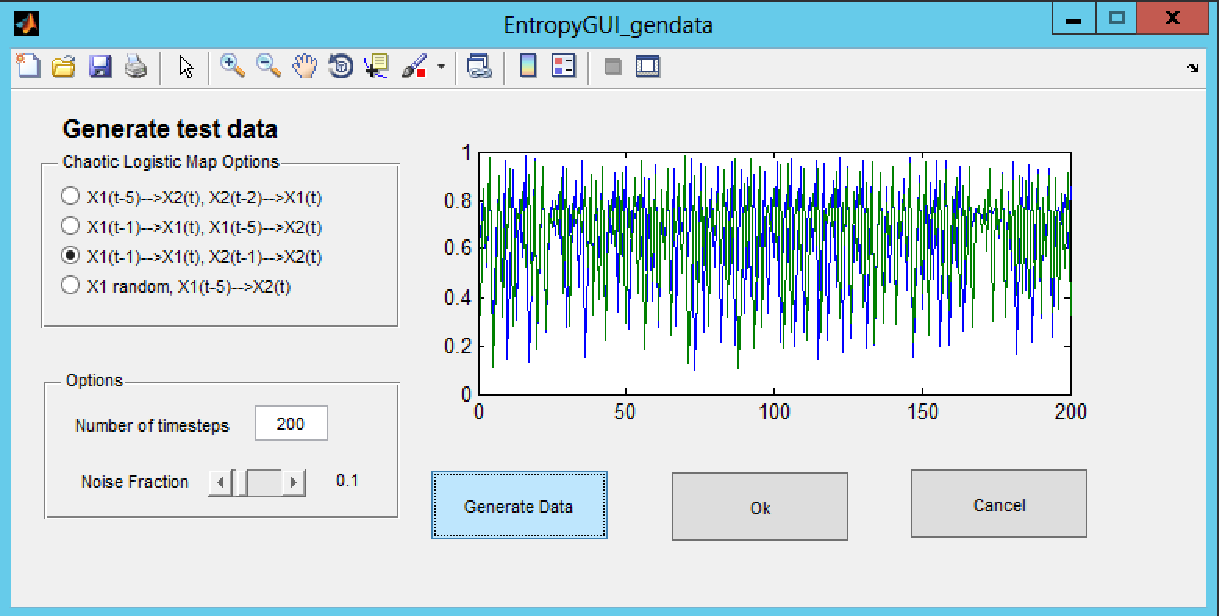
\includegraphics[scale=.5]{Image_GenData.pdf}
\caption{Example generated chaotic logistic test data with 0.1 noise (random component).}
\end{center}
\end{figure}

Alternatively to loading a time series data set, the \textbf{Generate Data} option generates a 2-node chaotic logistic time series data set for one of four different forcing cases: 

\begin{enumerate}
\item{Feedback forcing, where $X1$ and $X2$ drive each other:
\begin{align}
X2(t) = 4X1(t-5)[1-X1(t-5)] \\
X1(t) = 4X2(t-2)[1-X2(t-2)]
\end{align}
}

\item{$X1$ drives itself via the chaotic logistic equation and also drives $X2$:

\begin{align}
X2(t) = 4X1(t-5)[1-X1(t-5)] \\
X1(t) = 4X1(t-1)[1-X1(t-1)]
\end{align}
}

\item{$X1$ and $X2$ are independent, each driven by the chaotic logistic equation:

\begin{align}
X2(t) = 4X2(t-1)[1-X2(t-1)] \\
X1(t) = 4X1(t-1)[1-X1(t-1)]
\end{align}
}

\item{$X1$ is a uniform random variable, and drives $X2$ through the chaotic logistic equation:

\begin{align}
X2(t) = 4X1(t-5)[1-X1(t-5)] \\
X1(t) = U(0,1).
\end{align}
}

\end{enumerate}

For any case, the noise fraction slider bar for $0 \le \epsilon_z \le 1$ can be altered to add a degree of randomness into every node.  For example, $\epsilon_z =1$ generates 2 independent uniform random nodes.  

\subsection{Options}

\begin{figure}[h!]\label{fig:start}
\begin{center}
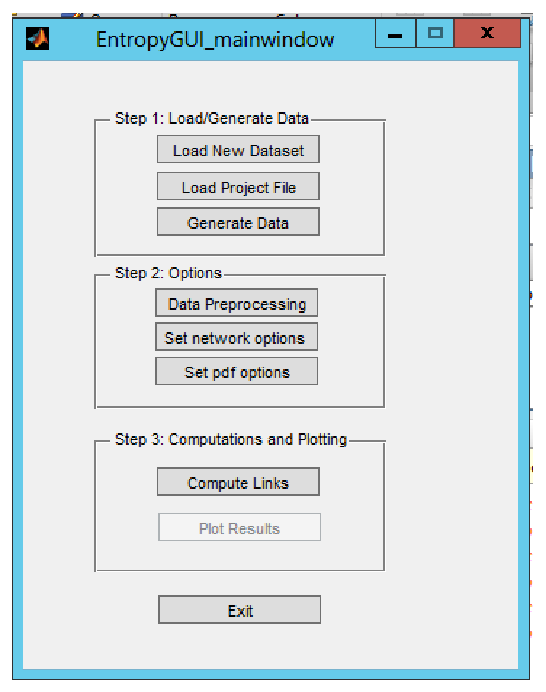
\includegraphics[scale=.5]{Image_Main_PreComputeLinks.pdf}
\caption{Main TIPNet screen.  A dataset, project file, or generated data must be loaded before continuing with options.}
\end{center}
\end{figure}

After loading a project file, new data file, or generated test data, there are three buttons to alter network parameters and properties from default values.  These options include \textit{pdf} estimation methods, network run options, and time-series pre-processing.

\subsubsection{Pre-Processing Options}
Each timeseries variable $X$ is automatically normalized between (0,1) as follows:

\begin{equation}
X_norm = \frac{(X-X_{min})}{X_{max}-X_{min}}
\end{equation}


\begin{figure}[h!]\label{fig:preprocess}
\begin{center}
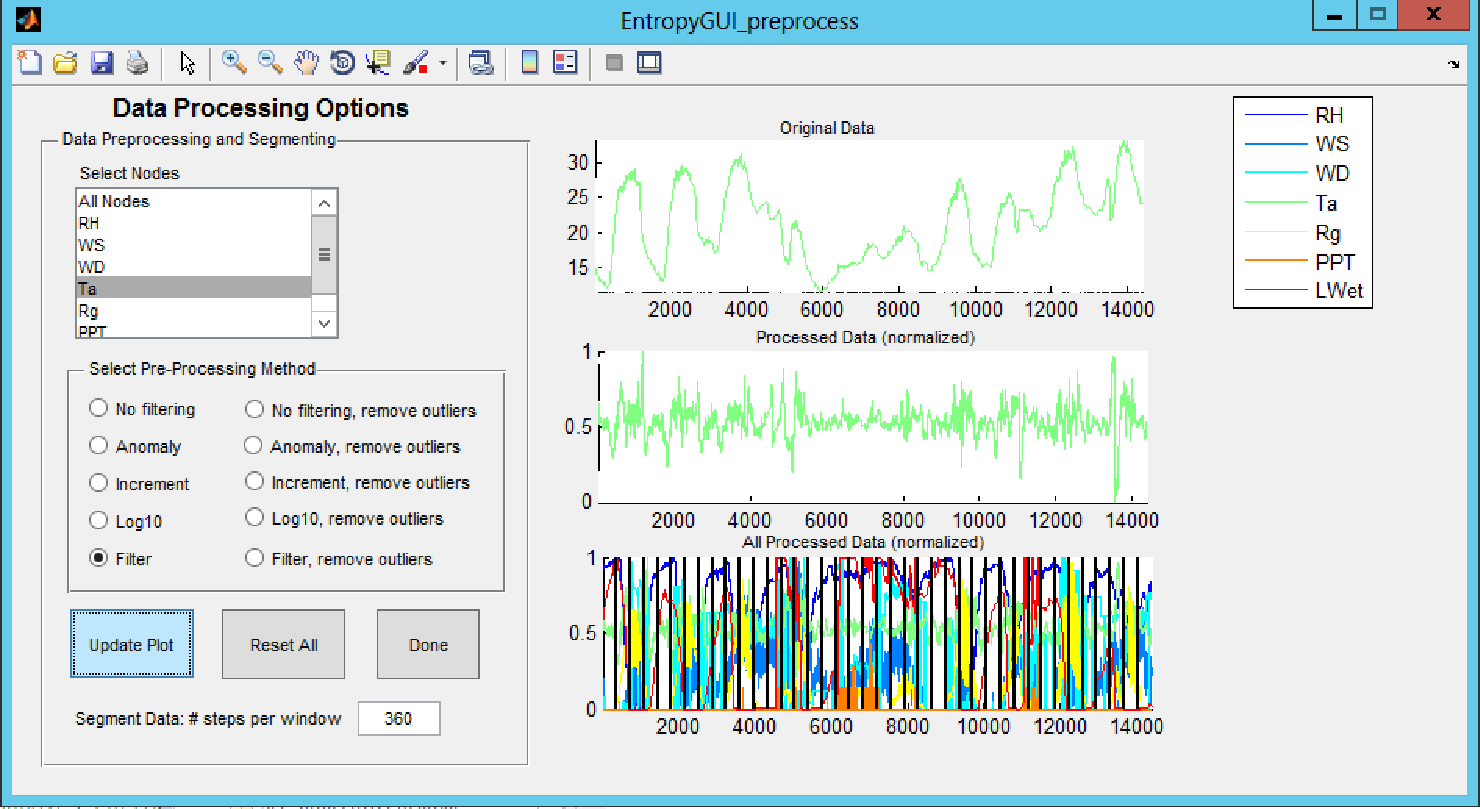
\includegraphics[scale=.5]{Image_Preprocess.pdf}
\caption{Data preprocessing screen.  Weather station data here has been segmented into 360 minute (6 hour) time segments as shown by black lines in bottom plot.  Nodes can be pre-processed individually or as a group.}
\end{center}
\end{figure}

Then, there are 5 types of data filtering or altering.  For each type, there is an option to remove or not remove outliers.

\begin{description}
\item[No Filtering] This option reverts the data to the original normalized data set.

\item[Anomaly] For data that exhibit diurnal or seasonal cycle, the X-day anomaly is the difference between the value at a certain time (e.g. 12:00 noon on Day 100) and the mean value at that time on the X surrounding days (e.g. 12:00 noon on Days 95-105 for a 10-day anomaly). The anomaly can only be computed for 1 variable at a time, and the user must check on the time step and units of the data (minutes, days) and units of the desired anomaly (days, years).  The anomaly of the originally loaded data is then normalized to a (0,1) range.


\begin{figure}[h!]\label{fig:anom}
\begin{center}
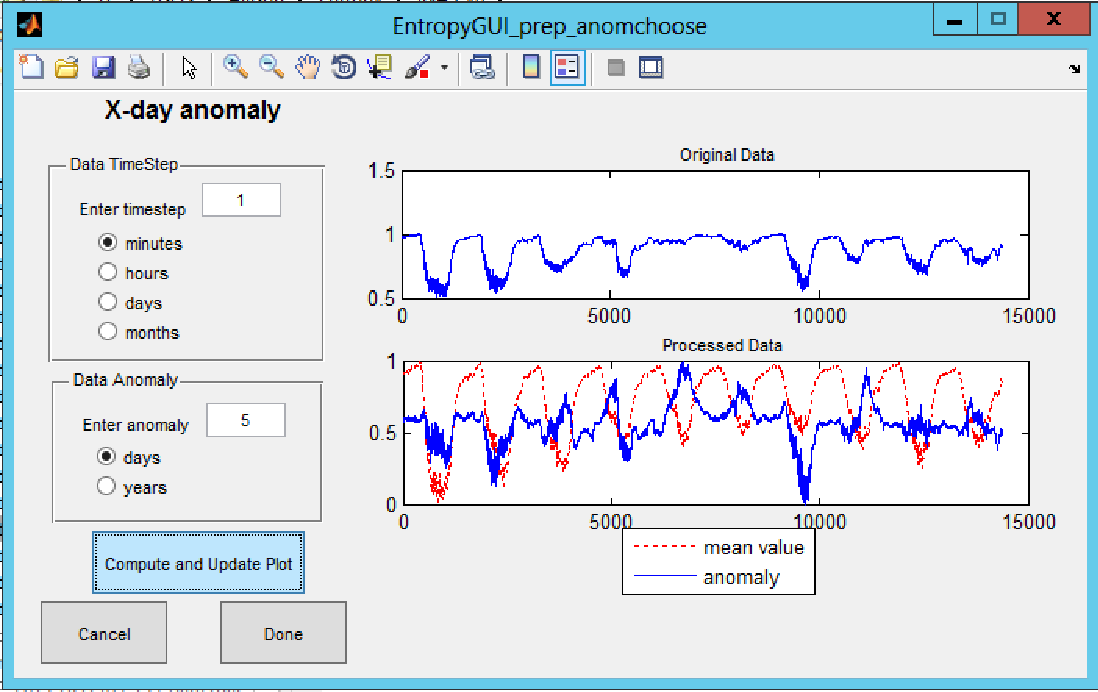
\includegraphics[scale=.5]{Image_AnomalyRH.pdf}
\caption{5-day anomaly of 1-minute resolution Relative Humidity data}
\end{center}
\end{figure}

\item[Increment] For data where an increase or decrease may be more relevant than an actual value (e.g. a population variable).  This changes the data as follows
\begin{equation}
X(t) = X(t)-X(t-1)
\end{equation}


\item[Log 10]: This takes the base 10 logarithm for skewed input data (e.g. flow rate data)

\item[Filter] For a single variable at a time, this option applies a Butterworth Filter to the data for a high-pass or low-pass filter to preserve or omit short-term fluctuations.  This can be used to (a) omit the diurnal and/or seasonal cycle with a high-pass filter (b) omit noise with a low-pass filter.

\begin{figure}[h!]\label{fig:filterhp}
\begin{center}
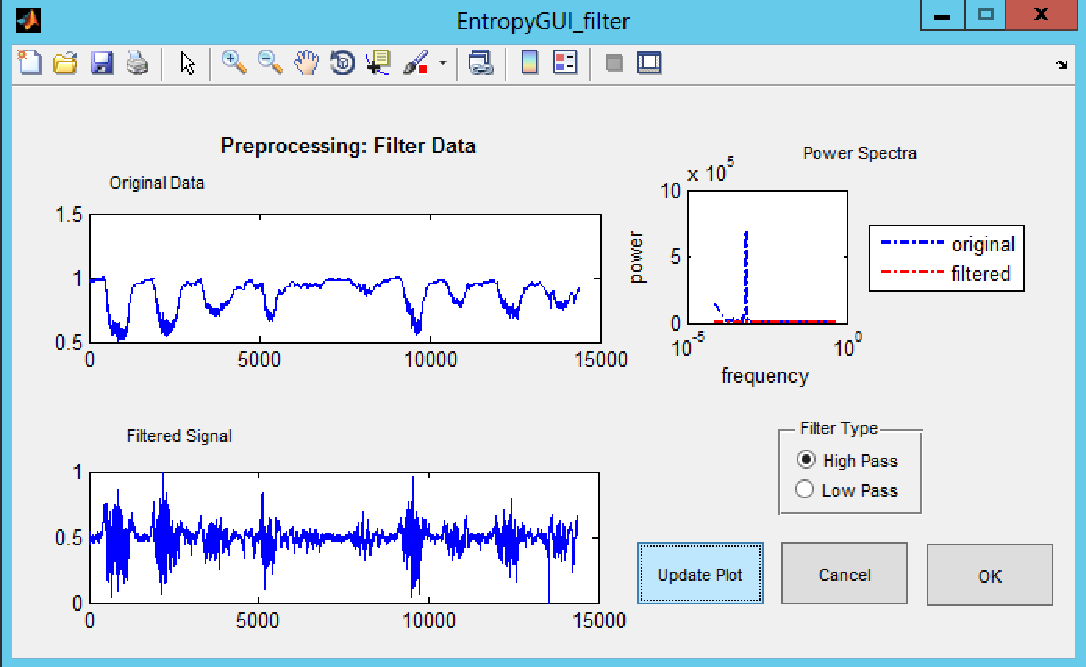
\includegraphics[scale=.5]{Image_FilterRH_hp.pdf}
\caption{High pass filter applied to Relative Humidity data}
\end{center}
\end{figure}


\begin{figure}[h!]\label{fig:filterlp}
\begin{center}
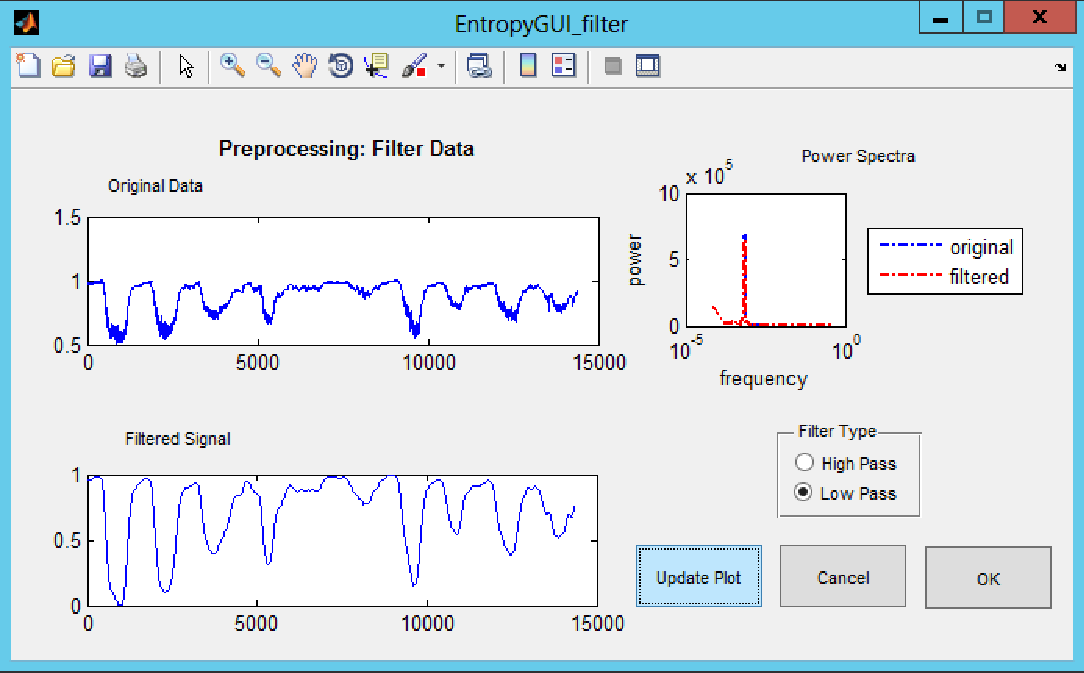
\includegraphics[scale=.5]{Image_FilterRH_lp.pdf}
\caption{Low pass filter applied to Relative Humidity data}
\end{center}
\end{figure}



\end{description}

For each option, outlier removal is performed after the operation (e.g. after taking the logarithm or increment).  Outliers, data points that lie above $X_{75} +1.5IQR$ or below $X_{25}-1.5IQR$, are set to the values $X_{75} +1.5IQR$ or $X_{25}-1.5IQR$, respectively rather than being removed.  Removal of outliers would impact the time dependencies by removing a time-step of the specified variable.  Any outlier removal via gap-filling or other methods should be done prior to loading a dataset.

Finally, to partition a long time-series data sets into multiple segments, the segment length can be changed.  This option results in computation of one network for each time-series segments, and is useful to compare before-after scenarios or to consider the evolution over time of interactions.

\subsubsection{Network Options}

\begin{figure}[h!]\label{fig:start}
\begin{center}
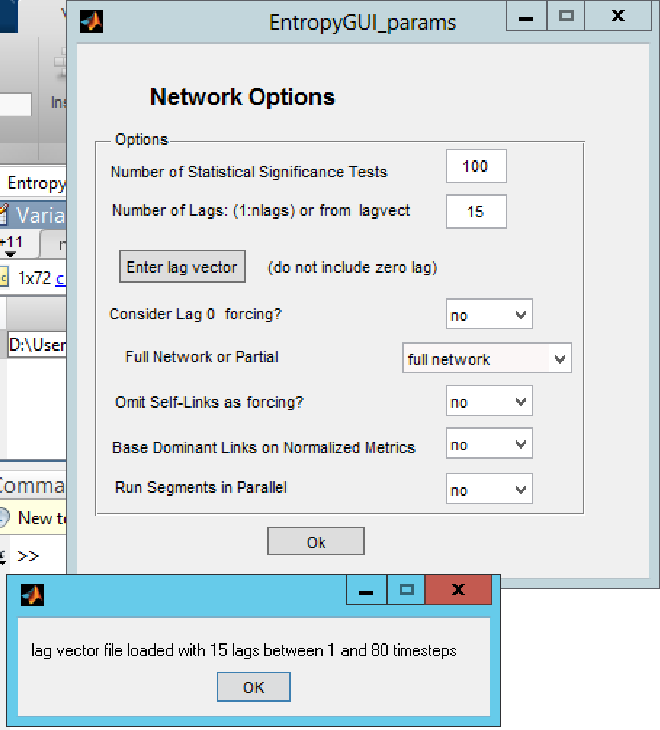
\includegraphics[scale=.5]{Image_NetworkOptions_LoadLagVect.pdf}
\caption{Network Options screen.  When a \textit{lagvect.mat} file is chosen, a verification message appears if the file is properly loaded. Alternatively, the number of lags can simply be entered in the text box for consecutive lag times.}
\end{center}
\end{figure}

The Network Options screen contains several options:

\begin{description}
\item[Statistical Sig Tests:] The shuffled surrogates method is used to determine statistical significance of each computed $I(X_1;X_2)$ value.  The default number of significance tests is 100.
\item[Number of Lags:] The number of lags for which lagged information measures are to be computed as $\tau = 1...\text{nlags}$.
\item[Enter Lag Vector:] Alternatively to specifying a number of consecutive lags, load a .mat file called lagvect.mat with a vector of lags named lagvect, containing lags.  This can be used to compute lags at intervals, for example lagvect = [5 10 15 30 60 120] to compute network measures at only 6 time lags but for different lag times than 1-6.  A \textit{lagvect.mat} file is provided in the folder \textit{UserData}, and should be overwritten as needed.  The lag vector shoudl consist of non-negative integers, should not include zero (see next point).

\item[Lag Zero Forcing:]  By default, zero-lag or instantaneous mutual information is not considered as a dominant link that can be redundant, synergistic, or unique with any other link.  To include zero-lag forcing (e.g. if the time step is such that X may be expected to drive Y at a time scale much lower than the time step), change this option to \textit{Yes}.
\item[Network Run Option:] By default, the program will perform all computations for mutual information, transfer entropy, and information decomposition as described in the previous section.  To only compute individual node entropy or mutual information, change this option as appropriate.  Note: the \textbf{Plot Results} viewer will not function if this option is altered.
\item[Omit Self-Links:] By default, node $X$ is considered as a potential source to itself, and a detected link $I(X(t-\tau);X(t))$ may be unique, synergistic, or redundant when another link to $X$ is considered.  To omit these ``self'' links, change this option to \textit{Yes}.
\item[Run Segments in Parallel:] If your data set is segmented into multiple time series in the \textbf{Pre-Processing Options} and your computer can run parallel code in Matlab (parfor loops), enable this to run segments in parallel.
\end{description}

\subsection{PDF options}
All information measures computed in this program are based on 1D, 2D, and 3D \textit{pdf}s.  This screen allows you to view these \textit{pdf}s and alter parameters.



\begin{figure}[h!]\label{fig:pdf_fixed}
\begin{center}
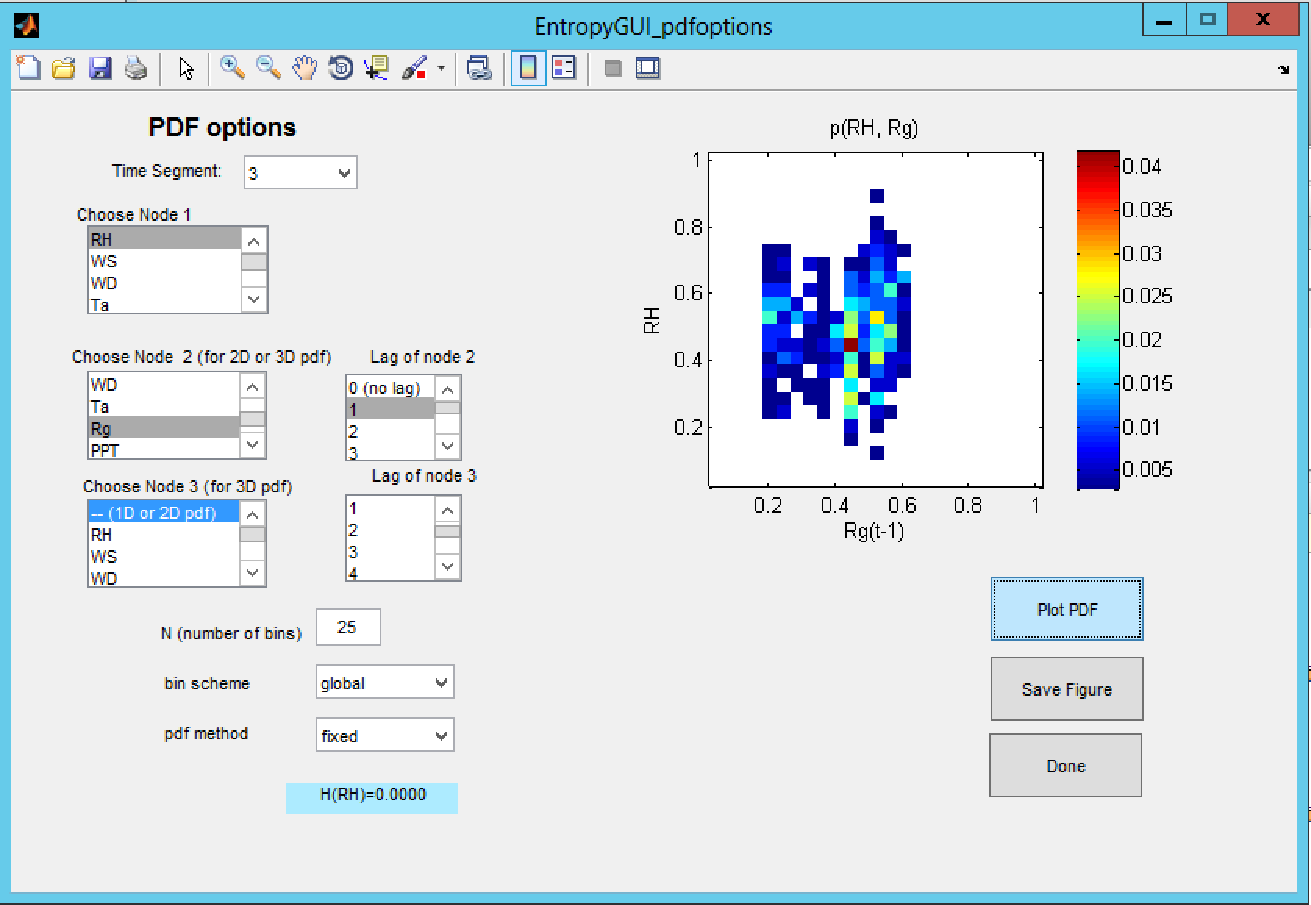
\includegraphics[scale=.5]{Image_PDF_RHTA_fixed.pdf}
\caption{\textit{Pdf} of RH and lagged Ta for a specific segment using global binning, fixed bins and $N=25$.  Red color indicates higher value of $p(RH,Ta(t-1))$}
\end{center}
\end{figure}

\begin{figure}[h!]\label{fig:pdf_KDE}
\begin{center}
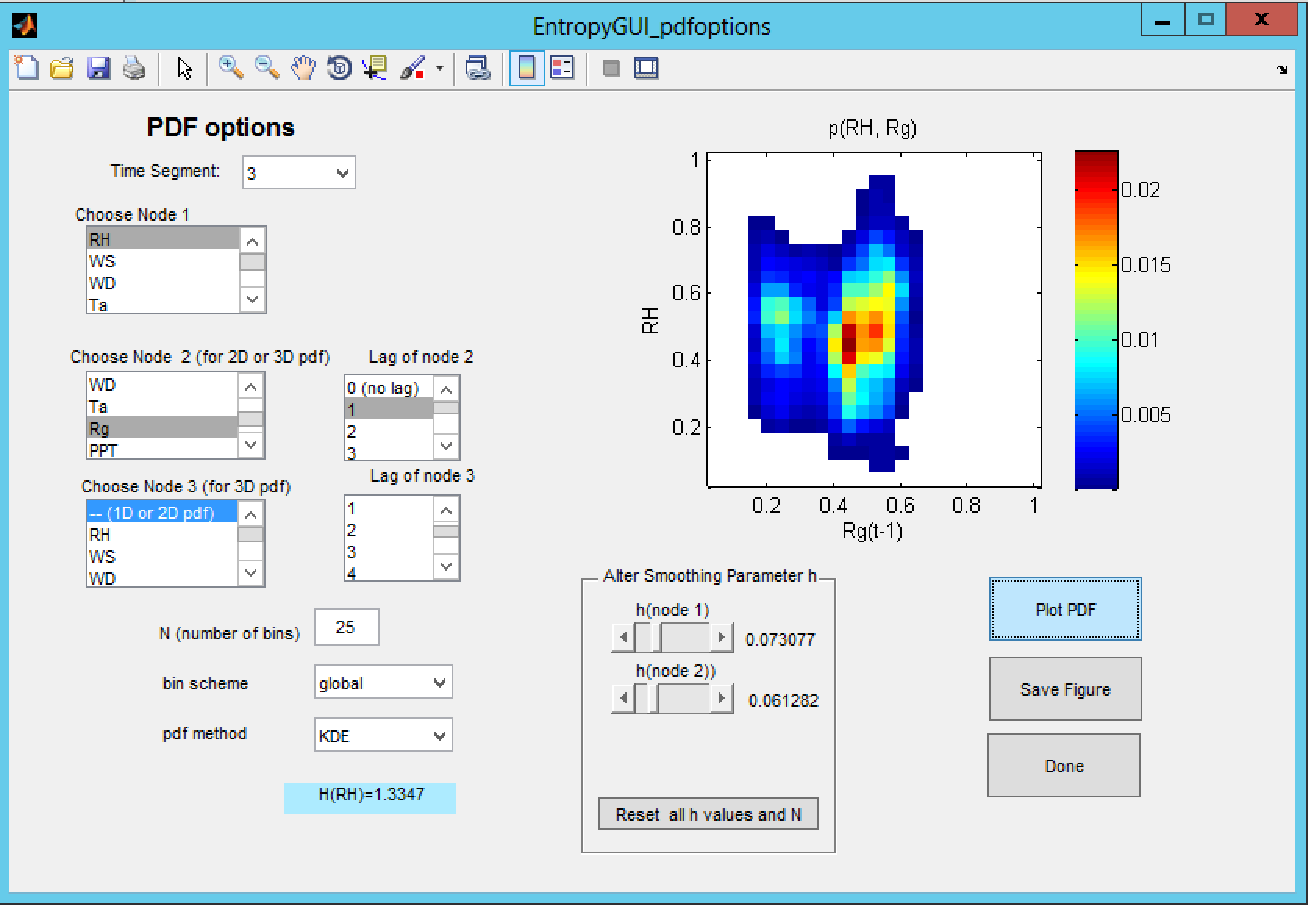
\includegraphics[scale=.5]{Image_PDF_RHTA_KDE.pdf}
\caption{\textit{Pdf} of RH and lagged Ta for a specific segment using global binning, KDE and increasing $h$ smoothing parameters slightly for both nodes.}
\end{center}
\end{figure}

\begin{figure}[h!]\label{fig:pdf_3D}
\begin{center}
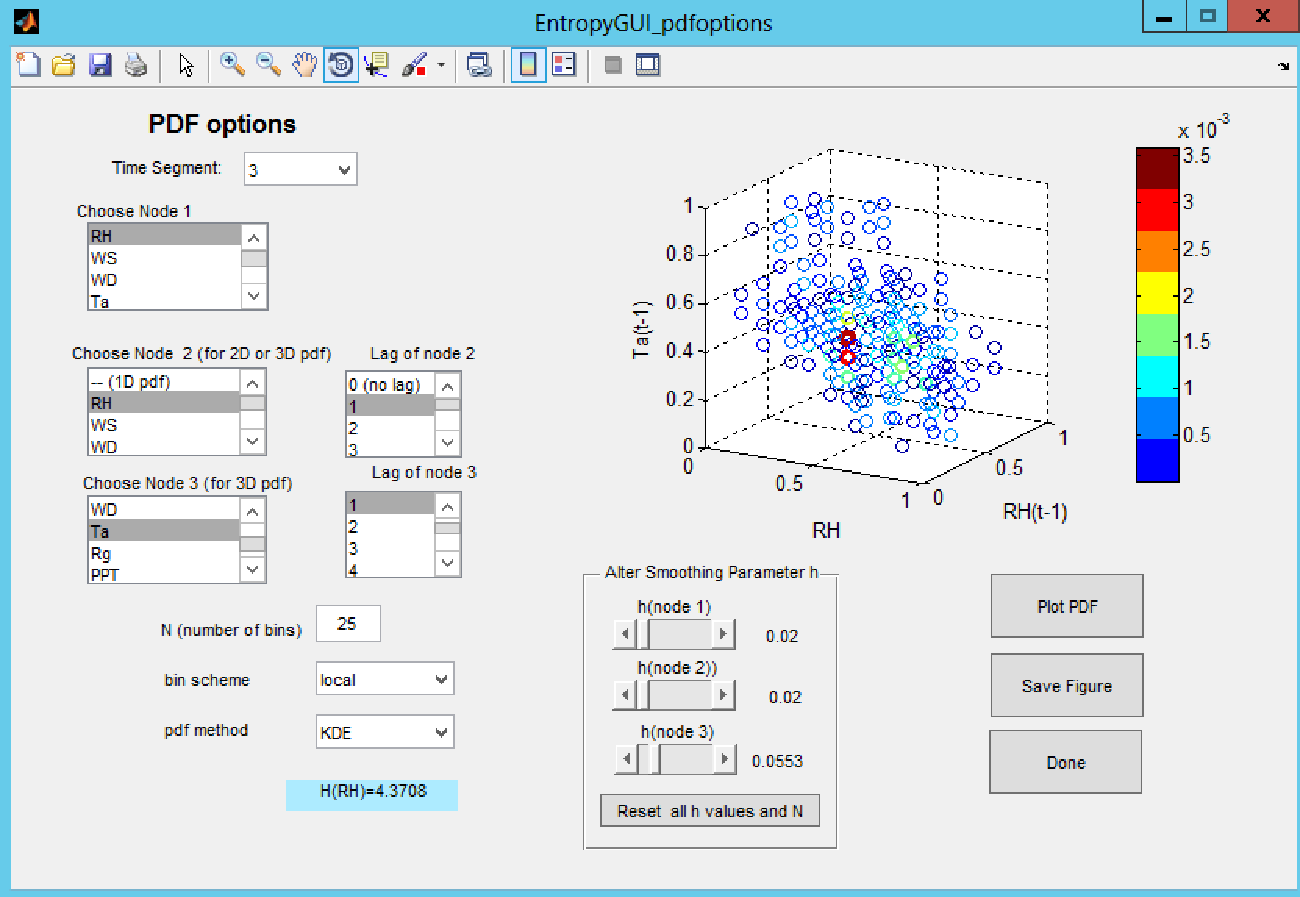
\includegraphics[scale=.5]{Image_PDF_3D.pdf}
\caption{3D \textit{Pdf} of RH, lagged Ta, and lagged RH for a specific segment using KDE method.  Red color indicates higher value of $p(RH,Ta(t-1),RH(t-1))$}
\end{center}
\end{figure}

\begin{description}
\item[Time Segment] For data sets that have been segmented in \textbf{Pre-Processing Options}, choose segment to view \text{pdf}.

\item[Choose nodes and lags] Choose 1,2 or 3 nodes to view 1D, 2D, or 3D \textit{pdf}, respectively. To view lagged \textit{pdf}, choose lag for second and third nodes.  A 1D \textit{pdf} will appear as a bar chart where the height of each bar corresponds to $p(x)$.  A 2D \textit{pdf} will appear as a color scaled image where the color corresponds to $p(x,y)$.  A 3d \textit{pdf} will appear as a 3D point cloud, where a point represents a $p(x,y,z)>0$. 

\item[N] Number of bins or locations at which to compute \textit{pdf}.  The default value is $N=25$, and $N$ can range up to 100.  
\item[pdf method] Choose between the KDE method and fixed bin method (default).  For the KDE method, a box will appear in which the smoothing parameter $h$ can be altered.  A larger $h$ value for a node results in a smoother \textit{pdf}.  Once $h$ is changed for a node, it is updated in the \textbf{mi.KDEparams} structure.
\item[bin scheme] For segmented data, a global bin scheme (default) scales the data between the global minimum (0) and maximum (1) values.  A local bin scheme scales the data for each segment separately between the minimum and maximum values in that segment.
\end{description}



After selecting nodes and/or altering parameters, clicking \textbf{Plot PDF} will update the \textit{pdf} plot accordingly.  When the KDE method is selected, the \textbf{Reset all h values and N} button will reset any previously altered smoothing parameters to the default values and set $N=25$.  Clicking \textbf{Done} will save any altered parameters.

\subsection{Network Computations and Plotting}

Once all options have been selected as desired, click \textbf{Compute Links} to construct the temporal information networks.

If the Parallel option is turned off (default option in \textbf{Network Options}), a timer window will appear for each segment.  For large data sets (typically greater than 1000 data points per segment, more than 20 nodes, or many segments), this could take several minutes to initialize and up to multiple hours to complete. When the Parallel Option is turned on, a progress bar will appear in the Matlab command window.  When all computations are finished, the output is saved in the previously created project file in a structure called \textit{entropy}.

\begin{figure}[h!]\label{fig:timerbar}
\begin{center}
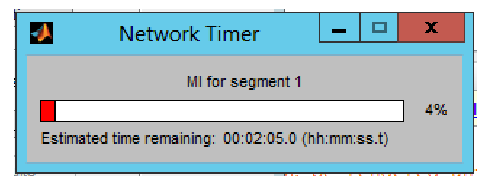
\includegraphics[scale=.5]{Image_timerbar.pdf}
\caption{Timer bar will appear for each segment of data set.}
\end{center}
\end{figure}

Click \textbf{Plot Results} to view network figures.  

\begin{figure}[h!]\label{fig:plotdata}
\begin{center}
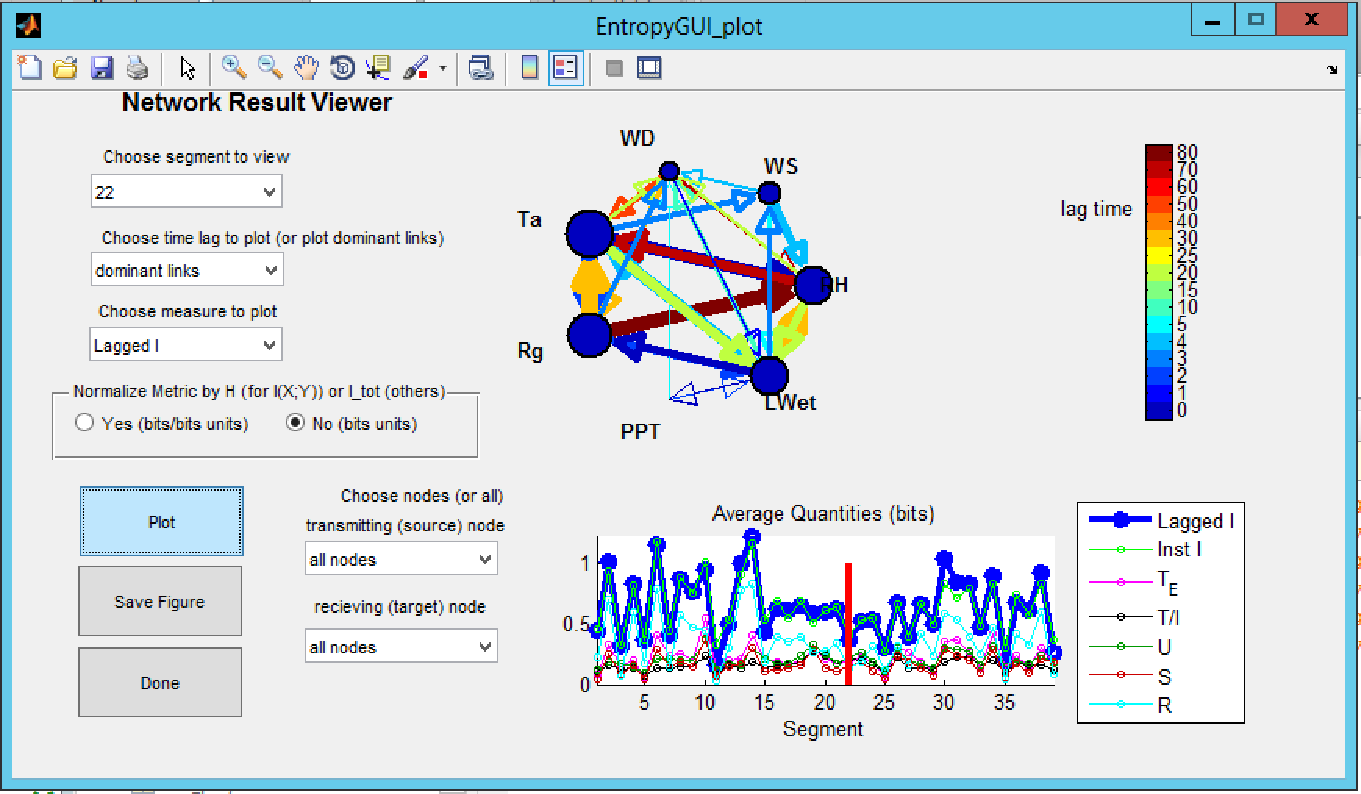
\includegraphics[scale=.5]{Image_PlotResults.pdf}
\caption{Result Viewer, showing Segment 20 lagged information network statistics for all nodes}
\end{center}
\end{figure}

The network circle plots contain each node and depict several information measures and associated time lags and strengths.  The arrow indicates directionality (source to target), the color indicates time lag of detected link, and the line width indicates the strength of the link.  The node size and color correspond to the ``self''-link properties, which may or may not be relevant depending on the selection of \textbf{Omit Self Links} in the Network Options.   The time series or point plot below the circle network shows each segment (for 1 or more segments) and the total values (averages) for 6 information measures.

\begin{description}
\item[Choose Segment] This list box is only visible if the data set has been partitioned into multiple segments in the \textbf{Pre-Processing Options}.
\item[Choose Time Lag] For lagged mutual information only, the value $I(X(t-\tau);Y(t))$ can be plotted for individual values of $\tau$ as defined in the lag vector (\textit{mi.lagvect}).  For all other measures, only the dominantly detected lags are shown in the circle network plot.
\item[Choose Measure]  6 measures can be plotted as described in the previous section
\item[Normalize]  To depict links normalized by entropy $H(X)$ (for lagged $I$) or total information $I_tot$ (for all other values except $T/I$ which is already normalized), check \textit{Yes}.  Otherwise, values plotted are in units of \textit{bits}.
\item[Choose nodes (or all)] Select a specific node pair to view only statistics for that link, or a single source or target node to view out-going or incoming links, respectively.
\end{description}

\bibstyle{mdpi.bst}
\bibliography{InfoPaper_Refs2}

\end{document}